\documentclass[12pt, twoside]{article}
\usepackage[letterpaper, margin=1in, headsep=0.5in]{geometry}
\usepackage[english]{babel}
\usepackage[utf8]{inputenc}
\usepackage{amsmath}
\usepackage{amsfonts}
\usepackage{amssymb}
\usepackage{tikz}
\usepackage{yhmath}
\usetikzlibrary{quotes, angles}
\usepackage{graphicx}
\usepackage{enumitem}
\usepackage{multicol}

\newif\ifmeta
\metatrue %print standards and topics tags

\title{Regents Geometry}
\author{Chris Huson}
\date{March 2022}

\usepackage{fancyhdr}
\pagestyle{fancy}
\fancyhf{}
\renewcommand{\headrulewidth}{0pt} % disable the underline of the header
\raggedbottom

\fancyhead[LE]{\thepage}
\fancyhead[RO]{\thepage \\ Name: \hspace{4cm} \,\\}
\fancyhead[LO]{BECA / Dr. Huson, Mr. Segal / Geometry\\* Unit 13: Data analysis\\* 31 May 2022}

\begin{document}
\subsubsection*{13.1 Classwork: Sector calculations}
\emph{Unless otherwise instructed, round final answers to three significant figures.}\\
\textbf{Formulas}\\
Where $r$ is the circle's radius, $D$ its diameter, and $\theta$ is the sector angle measured in degrees.
  \[\text{Circle circumference: } \;\; C=\pi D = 2\pi r\]
  \[\text{Length of an arc: } \hspace{1cm} l=\frac{\theta}{360} \times 2\pi r\]
  \[\text{The area of a circle: } \hspace{1.6cm}  A=\pi r^2\]
  \[\text{Area of a sector: } \hspace{1cm}  A=\frac{\theta}{360} \times \pi r^2\]
  \vspace{0.25cm}
\begin{enumerate}
\item Given the circle $O$ centered at the origin with radius $r=10$ and $A(10,0)$, $B(0,10)$.
  \begin{enumerate}[itemsep=1.75cm]
    \begin{multicols}{2}
    \item Find the circumference of circle $O$.
    \item Find the area of the circle.
    \item Find the length of the arc in the first quadrant (a quarter of the circle).
      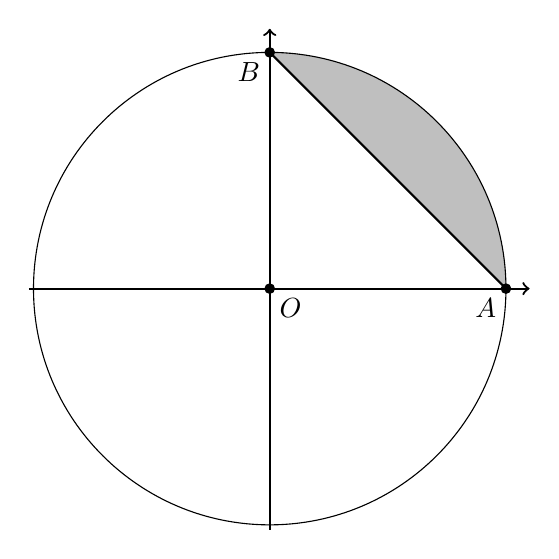
\begin{tikzpicture}[scale=.3]
        \fill [lightgray] (0,10)--(0:10) arc (0:90:10)--(0,10);
        \draw [thick, ->] (-10.2,0) -- (11,0);% node [below right] {$x$};
        \draw [thick, ->] (0,-10.2)--(0,11);% node [left] {$y$};
        \draw (0,0) circle [radius=10] node[below right]{$O$};
        \draw [fill] (0,0) circle [radius=0.2];
        \draw [fill] (10,0) circle [radius=0.2]node[below left]{$A$};
        \draw [fill] (0,10) circle [radius=0.2]node[below left]{$B$};
        \draw [thick] (10,0)--(0,10);
      \end{tikzpicture}
    \end{multicols}
    \item Find the area of the sector $AOB$ (quarter circle in the first quadrant).
    \item Find the area of the triangle $AOB$.
    \item Find the area of the segment $AB$ of circle $O$ (shaded area).
  \end{enumerate}

\newpage
\item Sector $AOB$ of circle $O$ has a central angle of $30^\circ$ with $A(10,0)$, $B(8.66,5)$.
\begin{multicols}{2}
  \begin{enumerate}[itemsep=1.6cm]
      \item Find the area of the sector $AOB$.
      \item Find the area of the triangle $AOB$.
      \item Find the area of segment $AB$ (shaded area).
      
      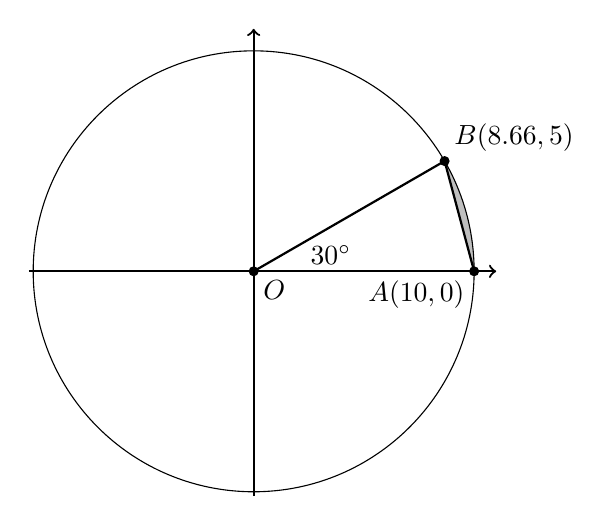
\begin{tikzpicture}[scale=.28]
        \fill [lightgray] (30:10)--(0:10) arc (0:30:10)--(30:10);
        \draw [thick, ->] (-10.2,0) -- (11,0);% node [below right] {$x$};
        \draw [thick, ->] (0,-10.2)--(0,11);% node [left] {$y$};
        \draw (0,0) circle [radius=10] node[below right]{$O$};
        \draw [fill] (0,0) circle [radius=0.2];
        \draw [fill] (10,0) circle [radius=0.2]node[below left]{$A(10,0)$};
        \draw [fill] (30:10) circle [radius=0.2]node[above right]{$B(8.66,5)$};
        \draw [thick] (0,0)--(30:10)--(10,0);
        \node at (3.5,0.75){$30^\circ$};
      \end{tikzpicture}
  \end{enumerate}
\end{multicols} \vspace{1cm}

\item Sector $AOB$ of circle $O$ has a central angle of $30^\circ$ with $A(10,0)$, $B(5,8.66)$.
\begin{multicols}{2}
  \begin{enumerate}[itemsep=1.6cm]
      \item Find the area of the sector $AOB$.
      \item Find the area of the triangle $AOB$.
      \item Find the area of segment $AB$ (shaded area).

      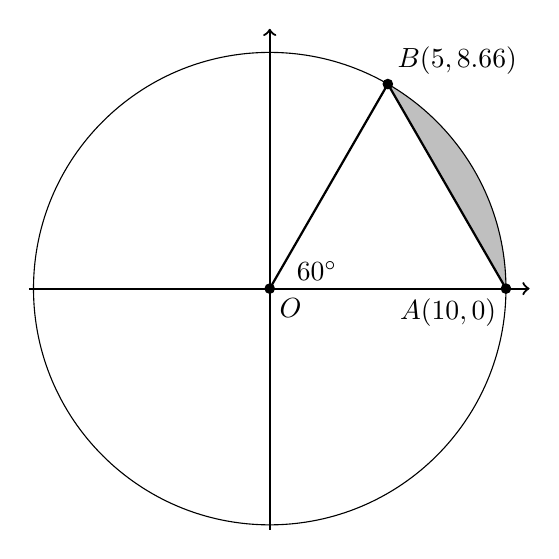
\begin{tikzpicture}[scale=.3]
        \fill [lightgray] (60:10)--(0:10) arc (0:60:10)--(60:10);
        \draw [thick, ->] (-10.2,0) -- (11,0);% node [below right] {$x$};
        \draw [thick, ->] (0,-10.2)--(0,11);% node [left] {$y$};
        \draw (0,0) circle [radius=10] node[below right]{$O$};
        \draw [fill] (0,0) circle [radius=0.2];
        \draw [fill] (10,0) circle [radius=0.2]node[below left]{$A(10,0)$};
        \draw [fill] (60:10) circle [radius=0.2]node[above right]{$B(5,8.66)$};
        \draw [thick] (0,0)--(60:10)--(10,0);
        \node at (2,0.75){$60^\circ$};
      \end{tikzpicture}
  \end{enumerate}
\end{multicols} \vspace{1cm}

\end{enumerate}
\end{document}
